\documentclass[10pt]{article}
\linespread{1.2}
\setlength{\parskip}{1.25ex}
\usepackage{xcolor}
\addtolength{\oddsidemargin}{-.875in}
\addtolength{\evensidemargin}{-.875in}
\addtolength{\textwidth}{1.75in}
\addtolength{\topmargin}{-.875in}
\addtolength{\textheight}{1.75in}
\usepackage[english]{babel}
\usepackage[utf8]{inputenc}
\usepackage{amsmath}
\usepackage{csquotes}
\usepackage{fancyhdr}
\usepackage{graphicx}
\usepackage{parskip}
%\usepackage{natbib}
\usepackage{pgfgantt}
\usepackage{lscape}
%\usepackage{pdfpages}
\usepackage{graphicx}
\usepackage{xcolor}
%\usepackage[minted]{tcolorbox}
\usepackage{hyperref}
\usepackage{wrapfig}
\usepackage{lastpage}
\pagestyle{fancy}
\fancyhf{}
\renewcommand{\footrulewidth}{1pt}
\cfoot{16018262}
\rhead{KF7004}
\rfoot{\thepage \hspace{0cm} of \pageref{LastPage}}
\usepackage{subcaption} 



\usepackage[style=authoryear-ibid,backend=bibtex]{biblatex}
\addbibresource{writing.bib}
\title{KF7004 – MComp Computing Research Project \\ MComp Research Proposal}
\author{16018262}
\date{Sept 22}


\begin{document}

\maketitle
\begin{center}
	Word count: 1584
\end{center}
\tableofcontents
\section{Research question}
%!TeX root=main.tex
%Can website log files be used to detect attacks.

%Is there enough data within website log files to detect attacks  on websites using a formulaic approach

A huristic analysis of website log files to detect attacks using a formulaic approach.
\section{Literature review}
%!TeX root=main.tex
%Background, Motivation and Relevance – literature review
 %•	Outline and critically discuss what relevant research has been undertaken in the past in your area of interest and why this project is necessary. 
%•	Outline and critically discuss why the research will be of value in the future and what the anticipated impact of the outcomes will be.
%•	Using supporting literature, set out and justify where your work will fit in the body of computing knowledge. Provide a diagram such as a mind map illustrating your position in the computing body of knowledge.
%\•	Outline why you want to undertake this work. Some areas to consider are personal motivation, skills set and career choices, a gap in the knowledge base and or relevance to your programme of study.

There have been multiple studies looking at website attacks but typically these have focused on single variable analysis e.g. CPU depletion. A good example, Erwin Adi has done a lot of research into Low-rate Denial of Service (LDoS) attacks. His primary paper looks at CPU depletion as an indicator of attack. In the same paper, Adi himself admits that this maybe a flawed technique for attack detection (\cite{Adi2016}). Most previous studies into detecting Low Bandwidth attacks only look at a single data point such as CPU. The present research proposes to look across multiple data points to detect attacks. 

Due to high volume of research in this area, high rate attacks don't pose the threat they used to, showing that preventative measures have been made. As Agrawal \& Tapaswi state "due to this huge volume of malicious traffic, such attacks can be easily detected. Thus, attackers are getting attracted towards the low-rate DDoS attacks. Low-rate DDoS attacks are difficult to detect due to their stealthy and low-rate traffic" (\cite{8794618}). Futhermmore in a study by \citeauthor{9016229} in 2020, they state that "Low-rate Denial of service (LDoS) attacks has become one of the biggest threats to the Internet, cloud computing platforms, and big data centers" (\cite{9016229}) showing the need for an effective attack detection tool.

Cloudflare statistics indicate that high rate DDOS attacks are increasing yearly however due to the protocols in place. High rate DDOS attacks aren't successful with there effects being easily mitigated (\cite{Q3attacks}). Whereas low rate attacks can be more easily disguised alongside more genuine use of the website thereby bypassing the protocols in place for high rate attacks. It's important to develop a system that is able to detect a wide variety of attacks in order to build a more comprehensive picture of low rate attacks and keep websites safer.

%reword?
The rate of request is not necessarily the only signal of an attack, the cumulative total over time should be considered. If for example if an IP address is constantly searching for login pages or back up files this could be an indication of suspicious behaviour. There is not a lot of data on low rate attacks and this could be a cause of concern and if we don't know how many attacks are happening it may indicate there is no detection method for the attacks. 

 %Tripathi researched attacks using website data and by recording traffic over a 14 hour period and proposed an anomaly detection technique that attempted to detect attacks by measuring the Chi squared (X\textsuperscript{\small2}) differential value between the expected traffic pattern, the result suggested attacks could be found with high accuracy (\cite{tripathi2018slow}). This study suggested that attacks could be detected with high levels of accuracy. This study utilised simulated data and therefore whilst theoretically sound  has limited application in the real word. 
 
 Tripathi proposed an anomaly detection technique that attempted to detect attacks by measuring the Chi squared (X\textsuperscript{\small2}) differential value between the expected traffic pattern, the result suggested that attacks could be found with high accuracy. Tripathi Collected 14 hours of HTTP/2 traffic, a fundamental issue with this being that the researcher simulated the data,(\cite{tripathi2018slow}) whilst theoretically sound there are no real world examples showing this to be effective. Therefore the data is not reliable because of the small time frame in which it was carried out and  it cannot be said for sure whether the changes in traffic would've occurred naturally making it hard to differentiate peaks in traffic or an attack. For this reason, \citeauthor{8500383} advocates for "the increased utilization of real-world data instead of simulated data." (\cite{8500383}). Therefore the present paper looks to use real data from multiple websites over an increased time-window, using data sciences techniques, to evaluate its efficiency. 

It has been suggested that storing large amounts of network traffic may be impractical (\cite{staniford2002practical}). However \citeauthor{9016229} states that  "A huge amount of network traffic can be collected, stored, organized and classified by big data analysis." (\cite{9016229}) Therefore if there is a need for a large amount of data, that may be impractical to store. One solution may be to look at the data already available to analyse and designing a suitable way to analyse that data. Most websites keep log files of who is accessing the website and activity history. Therefore theoretically the log files negate the need to collect extra data and may provide sufficient information to detect attacks. This method was tried by Smith (2020). However this only used a small data sample, but did have promising results as it was able to distinguish good traffic from bad traffic. 

Previous research looks at traffic flow in various ways, however it fails to take into account where that traffic is coming from, for example, most cyber attacks emanate from Russia and China, so the research is ignoring a key area that needs to be explored. The work done by Smith proposed a formula that took many factors  into account. The overall formula was defined as  \[risk = (orrcancesOfipLog \times 0.6) + ((requestRisk+responseRisk) \times 0.3) + (countryRisk \times  0.1) \] this formula was the first documented  attempt to look at multiple data points when detecting low rate attacks. However in Smith's conclusions he states that the network that the IP address comes from could potentially have a greater impact on the risk as due to VPN technology can change the country. Furthermore, the risk of a particular country only looks at the total number of attacks per country and Smith points out that  "the values used in the software are only based on the number of attacks per country" (\cite{smith}) therefore the overall calculation will be changed and the underlying risk assigned to each country will be assessed looking at attacks per head of population. In additon to the country, it would be useful to look at the network the IP comes from and build that into the calculation. 

\begin{wrapfigure}{R}{0.5\textwidth}
\label{web using h2}
    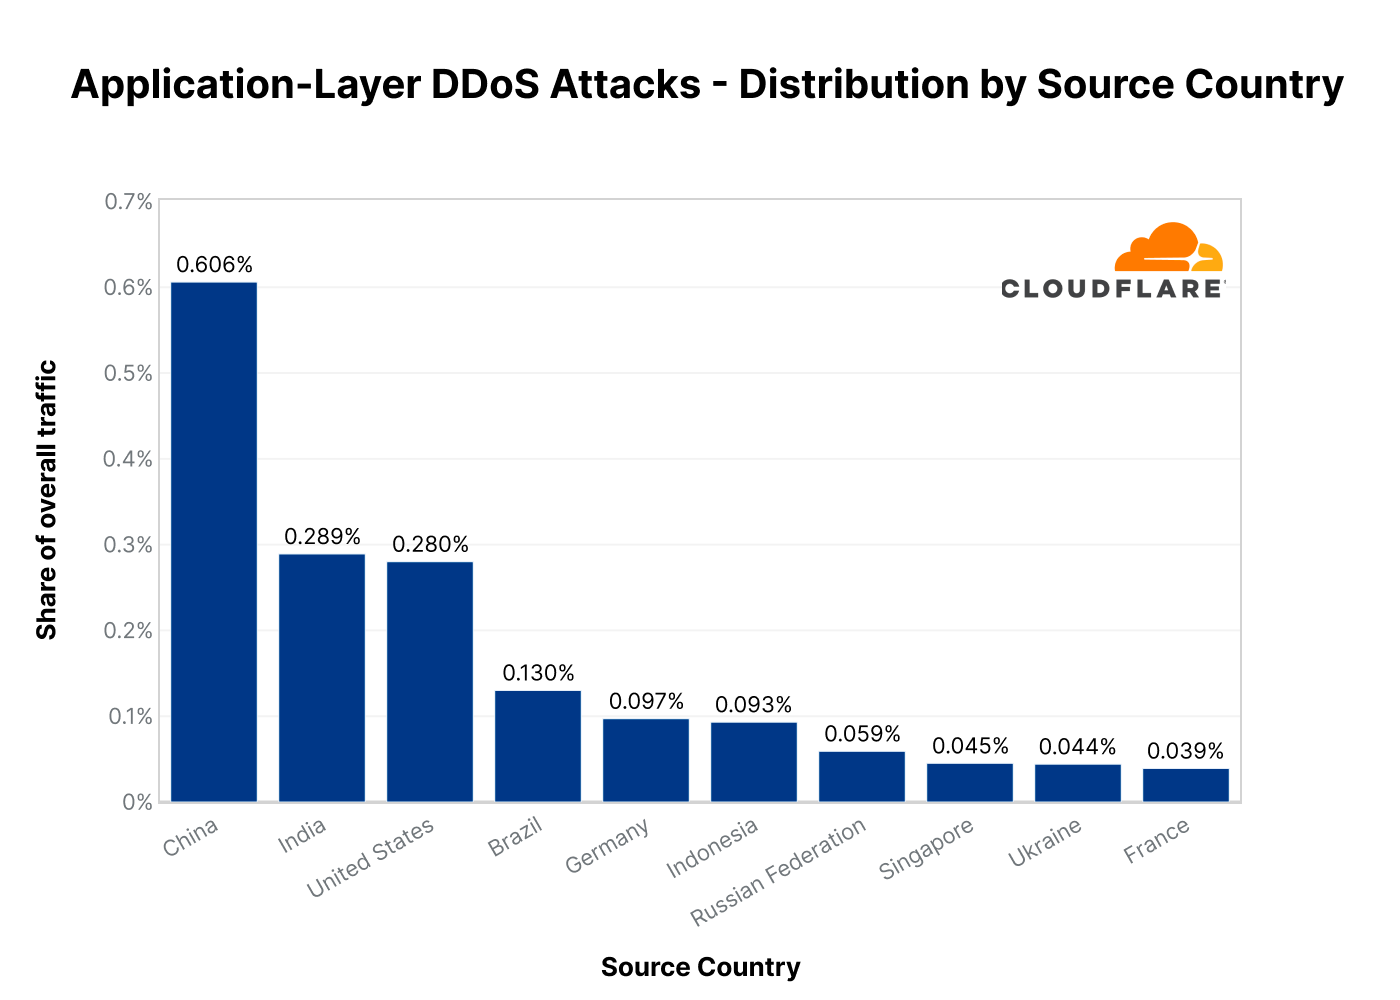
\includegraphics[width=88mm,scale=0.4]{images/CF q3.png} 
    \caption{Attacks by country according to Cloudflare}
\end{wrapfigure}
When looking at the risk from an individual country, the values used in the formula are only based on the historical number of attacks per country. While this is a good way to assess the risk of a country, this methodology could potentially have issues, for example, larger countries will statistically have more attacks than smaller countries. According to the Cloudflare DDoS threat report 2022 Q3, it was identified that the number of attacks coming from China- registered IP addresses increased by 29\% from the previous year. India has the second- largest source of HTTP DDoS attack traffic with an increase of 61\% (\cite{Q3attacks}).

 %According to Cloudflare in their DDoS threat report 2022, application layer DDoS attacks are mainly comming from China

%Tripathi put forward an approach in 2018 which as he suggests could accurately detect attacks. He came to this conclusion by using a sample of websites, and using the Chi squared method to detect low attacks by monitoring benchmarking. He concluded that using Chi squared differential it would be possible to detect an anomaly in traffic. The study took a sample of websites and attempted to detect low rate attacks by monitoring benchmarking and measuring the Chi squared (X\textsuperscript{\small2}) differential value between the expected and observed traffic pattern. Tripathi suggests this approach could detect attacks with high accuracy and may lead to future research to assess further HTTP/2 vulnerabilities, thus potentially mitigating these threat vectors with fixes. Tripathi indicated that although his detection method for attack traffic was successful; if HTTP/2 traffic data is encrypted it must then be decrypted before submitting traces to the detector. He suggested that this could be easily achieved with the aid of an intercepting proxy before forwarding to the target website responsible for handling HTTP/2 requests. It must be noted that most large companies are utilising this strategy to intercept traffic coming into their local network. (\cite{tripathi2018slow}). 

%Adi's 2017 work looked at some of the stealthier approaches that cyber attacks were using in order to bypass current detection methods. Adi and his team set up two models intended to simulate stealthy low rate DoS attacks which they called 'bots'. The investigation aimed to model attacks whose traffic continually consumed the victims computing resource, while still being stealthy enough to yield some false alarms via the target servers' 'learning' mechanisms. Adi constructed the attack 'bots' with four core factors for experimentation, these were number of threads, number of window\_update, stealthy factors and the delay between successive TCP connections. These two sets of Stealth models were tested against regular flash crowd traffic in an effort to differentiate the pattern. The experiment and subsequent analysis was successful in distinguishing a notable difference in the patterns of the number of packets carrying SYN flags per 1-second traffic instance between regular flashcrowd traffic and the simulated stealthy attacks (\cite{adi2017stealthy}). Since Adi's work there appears to be an implementation of the methodology proposed in their paper. For example, Cloudflare have been able to implement a defence mechanism against a SYN flood attack. The have created a program called 'gatebot' which monitors SYN packet requests and attempts to drop malicious SYN packets on the firewall layer (\cite{CFSYN}) the work does not refer to that of Adi's however the Cloudflare implementation does appear to use similar concepts. At the  time of writing this seems to be the only documented attempt of blocking SYN attacks.


%\subsection{revlantcy}
%The work is relevant due to the increasing number of websites increasing as nearly all businesses have a website. In the aftermath of remote working and lock downs E-commerce sites increased (CITE NEEDED) the types of attacks the study aims to detect can be hard to identify. Cloudflare notes in August  2022 that 

%attacks up on websites

%As websites become part of daily life the number of sites online is increasing as such there are more and more potential targets for attackers and more exploits are discovered, as attacks get more complex the is a need for different detection techniques.



%sim normal traffic
% then sim attack
\section{Aims}
The aim of this research is to build upon work carried out as part of a 2019 Study by Smith P. looking at a  formula approach to detecting risks posed by website traffic. The work done by Smith attempted to use website log files to detect suspicious activity on a website. This work will collect more data to prove the accuracy of this approach. As well as expanding the number of data points to detect attacks for example the network an IP belongs to and the user agents. The study by Smith P. only has a relatively small data set to it is hard to draw any wider conclusions about the accuracy of the technique proposed, therefore one of the primary aims of this study is to collect a wider data set. 
\subsection{Technical approaches and datasets}
%!TeX root=main.tex
The appoaches used in this work will be combing existing techiques in a new way. There will be a backend database that will hold data about the IP adresses of known bots so that thease can return a risk of 0. 

Another table will hold risks of http status coodes as  seen in apendix B, by keeping the values in the database table, it is easier to modify the risk. Furthermore another table holds signatures known attacks so that this can be run against the data. This makes it very quick to add new attacks to the formula.

The data analysed will be the apache common log format, this format conatains alot of technical information that will be beneficial to the formula. This data is stored in various data structures that can then be accessed to determine risk. In addition to this, the data from the database, for example the fragments of known bots are getting stored so that they can be cross referenced.  

To be able to identify the country of origin IP address, the maxmind geoip database is used then each country is assigned risk wieghting within a seperate database. The same process is used for the network risk.by using the maxmind databases, it ensures that the IP information is always up to date.
\section{Legal, social and ethical considerations}
%!TEX root = main.tex

One area of concern that may be a legal, social and ethical issue is whether the users of a website should be infoirmed that their IP address is being collected for analysis, this may have ethical repercusions as collecting IP addresses could potentially lead to individuals being identified. However most privacy policies on websites state that the IP will be collected to analyse trends, including one of thye websotes that has a agreed to donate data (\cite{PetersWebPrivacy}) and the system will only look at the network and country the IP belongs to.
%When thinking about an ethical way of collecting data one of the key questions is should the website data is collected say the data is being used for this?

%The main ethical issue is around collecting IP addresses this could potentially lead to individual being identified however the system will only look at the network the IP belongs to. 

Whilst the  consent of the website owners was  obtained the one ethical issue could be that  havent recieved consent from each of the individuals whose data I will be analysises. However if someone is trying to do malicious activity on a website they may want their data excluded from the analysis. Therefore it will be difficult to prove if it can pick up malicious activity. One social and ethical issue could be that entire countries are given a risk, however a user in that country may havce a legitimate reason to access a website. Therefore, to mitigate the risk of a social issue, the country that an IP belongs to will be given a minimal waiting in the overall formula. 

A full ethics  form can be found in appendix \ref{ethics}

One wider ethical issue of software like this could be if an attacker was able to figure out the formula they could work out how to get around the formula however that is a potential issue with all security, both digital and physical
\section{Scope}
%!TeX root=main.tex
The scope of this work is to build a small programme to analyse the data in website log files to determine if attacks can be detected. The main points of the work are:
\begin{itemize}
    \item identify how attack are evading current techniques 
    \item understand attack characteristics and update the fomula
    \item develop a formula that can detect and determine risk
\end{itemize}

This work will not automatically block IP addresses from accessing the website as that this may cause IP addresses to be incorrectly blocked \citeauthor{TargetedCyberSecurity}, pointed out that the unique 'human' ability to appraise the contextual features of a potential threat means that removing them from the loop of a security methodology is inadvisable. (\cite{TargetedCyberSecurity} ) So this work should be seen as a way to aid the decision making of website owners rather than make the decision for them. 

This work will not check the ability of people to use the software due to the fact it may be difficult to determine if it was the formula or user that identifies attack Bryman. states that "If we suggest that X causes Y, can we be sure that X is responsible for the variation for the Y and not something else". (\citeauthor{bryman_2016} \citeyear{bryman_2016};41). The work is fouced on proving if a formula can idenify attack traffic.

This work will not be looking to generate its own data as it may be easier to prove the accuracy of the formula on real data sets and  means the formula is written in ways that it will be possible to interpret real data.
\section{Risks}
\section{Risks}
One of the potential pit falls is differentiating potentials attacking with genuine user error. For example with low rate ddos attacks a login page could be repeatudly loaded however this could also be due to a user forgetting their password this is why the research needs multiplce indication of intent before classing this a attack.  

\printbibliography
\appendix
\section{Ethics} \label{ethics}
%
\includepdf[pages=-]{Website risk.pdf}
\newpage
\section{HTTP Status codes} \label{codes}
\vspace{5mm} %5mm vertical space
\begin{figure}[] \label{HTTP Status codes}
    \centering
     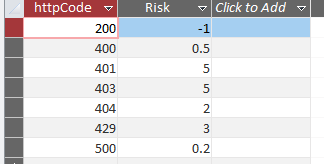
\includegraphics[width=170mm]{images/HTTP.png}
    \caption{HTTP Status codes}
    \label{fig:my_label}
\end{figure}
\end{document}
